\documentclass{beamer}

\mode<presentation> {
	\usetheme{Rochester}
	\setbeamertemplate{footline}[page number]
}

\usepackage{graphicx}
\usepackage{booktabs}

\title[Mind Map PIM]{Mind Map PIM}

\author{A-Cube-N}
\institute[UP]{
	Department of Computer Science, University of Pretoria
}
\date{\today}
\graphicspath{{pictures/}}

\begin{document}

\begin{frame}
	\titlepage
\end{frame}

\begin{frame}
	\frametitle{Overview}
	\tableofcontents
\end{frame}

\section{Concept}
	\subsection{Overview}
		\begin{frame}
		\frametitle{Project Overview}
		The Mind Map PIM is a system that pulls different social media platforms together and only displays information relevant to you at the current moment in your life in the form of a dynamic mind map.
		\end{frame}
	
	\subsection{What it is not}
		\begin{frame}
		\frametitle{What it is not}
		The Mind Map PIM is not a new social media platform. Rather it acts as a filter for current your current social media platforms. It uses intelligent algorithms to determine what information you would most likely want to see.
		\end{frame}
		
\section{Software Architecture}
	\subsection{Overview}
		\begin{frame}
		\frametitle{Software Architecture Overview}
		
		\end{frame}
		
	\subsection{Requirements}
		\begin{frame}
		\frametitle{Software Architecture Requirements}
		
		\end{frame}
		
	\subsection{Design}
		\begin{frame}
		\frametitle{Software Architecture Design}
		
		\end{frame}
		
	\subsection{Persistence}
		\begin{frame}
		\frametitle{Software Architecture Persistence}
		
		\end{frame}
		
	\subsection{Interface}
		\begin{frame}
		\frametitle{Software Architecture Interface}
			The system will be accessed via a web interface and an Android app. The mind map will be presented in a fashion similar to the way that musicroamer.com displays related music artists (see next slide).
			
			\begin{itemize}
				\item At the center is the root node.
				\item Each social media platform has a node going out from the root node.
				\item Relevant information is displayed about each platform.
				\item User can expand any node to find relevant information about that node.
			\end{itemize}
		\end{frame}
		
	\subsection{Interface}
		\begin{frame}
		\frametitle{Software Architecture Interface}
			\begin{figure}
				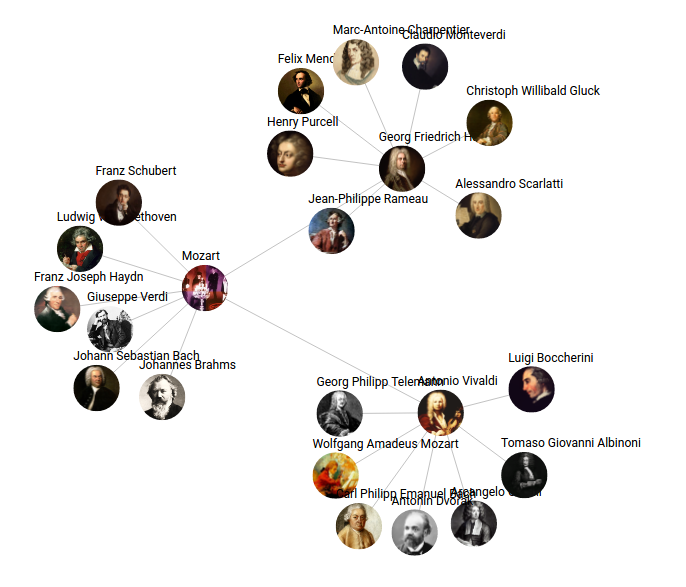
\includegraphics[scale=0.3]{musicroamer.png}
				\caption{Music Roamer layout of a music mind map}
			\end{figure}
		\end{frame}

\begin{frame}
	\Huge{\centerline{The End}}
\end{frame}

\end{document} 